\chapter{Determinantal Point Processes}
\label{chap_DPP}
We saw in \cref{chap_intro_coresets} the uniform bound on sample complexity of coresets. These bounds are based on Probabilistically Approximately Correct (PAC) learning theory results, where sample complexity bounds (with respect to $\delta$ and $\epsilon$) are known and tight in the i.i.d. framework. One could then be tempted to extend to the case where samples are drawn dependently.

Whereas the space of distributions for $m$ i.i.d samples has size that does not depend on $m$, the way $m$ samples can be correlated grows exponentially with $m$. In order to tackle this space of correlations, more recent results restricted to the cases of martingales or $\beta$-mixing processes, e.g. \cite{gao2016_learnability_beta_mixing}.

In the current chapter, we introduce Determinantal Point Processes (DPPs), another restriction of correlated sampling, which admits useful tractability properties, while still maintaining expressiveness into the sub-category of negatively correlated sampling. This negative correlation is expected to be a key property in order to perform better sampling complexity.

\section{Some intuition}

A Determinantal Point Processes (DPP) is a random sampling over subsets of a given ground set. Noticeably, its distribution is entirely encoded by a given positive kernel, which can be tuned to a range of specific contexts. In a sense, DPPs can be said to be the kernel machine of point processes, as they allow both tractability and flexibility. 

An essential characteristic of a DPP is that the occurrences of the element of the ground set are negatively correlated, i.e. the inclusion of one item makes the inclusion of other items less likely. The strengths of these negative correlations are derived from a kernel matrix that defines a global measure of similarity between pairs of items, so that more similar items are less likely to co-occur. As a result, DPPs assign higher probability to sets of items that are diverse.




\section{Definition}
Determinantal Point Processes are before all point processes, which can be described as processes for selecting a collection of mathematical points randomly located on a mathematical space. Formally, a point process $\PP{}{}$ on a ground set $\mathcal{X}$ is a probability measure over "point patterns" or "point configurations" of $\mathcal{X}$, which are subsets of $\mathcal{X}$. For instance, $\mathcal{X}$ could be a continuous region of the euclidean plane in which a scientist injects some quantum particles trapped into a potential well. Then $\PP{}{\left\{x_1, x_2, x_3\right\}}$ characterizes the likelihood of seeing these particles at places $x_1, x_2$, and $x_3$. Depending on the type of the particles, the measurements might tend to cluster together, or they might occur independently, or they might tend to spread out into space. $\PP{}{}$ captures these correlations.

In the following, we focus on discrete, finite point processes, where we assume without loss of generality that $\mathcal{X}=\begin{Bmatrix}
    x_{i} \mid i\in \intint{1}{n}
    \end{Bmatrix}$, in this setting we sometimes refer to elements of $\mathcal{X}$ as items. The discrete setting is computationally simpler and often more appropriate for real-world data.

In the discrete case, a point process is simply a probability measure on $2^{\mathcal X}$ i.e. the power set of $\PP{}{}$ i.e. the set of all subsets of $\mathcal{X}$. A sample from $\PP{}{}$ might be the empty set, the entirety of $\mathcal{X}$, or anything in between. 
\begin{definition}[Determinantal Point Process]
    \label{def_dpp}
    $\PP{}{}$ is called a determinantal point process if, when $\mathcal{S}$ is a random subset drawn according to $\PP{}{}$, we have, for every $A \subseteq \mathcal{X}$,
    \begin{equation}
        \PP{}{A \subseteq \mathcal{S}}=\operatorname{det}K_A
    \end{equation}
    for some real, symmetric matrix $K \in \RR^{n \times n}$ indexed by the elements of $\mathcal{X}$.
\end{definition}
Here, $K_A :=$ $\left[K_{x y}\right]_{x, y \in A}$ denotes the submatrix of $K$ indexed by elements of $A$, and we adopt $\operatorname{det}K_\emptyset=1$. Note that normalization is unnecessary here, since we are defining marginal probabilities that need not sum to $1$ .

Since $\PP{}{}$ is a probability measure, all principal minors $\operatorname{det}K_A$ of $K$ must be positives, and thus $K$ itself must be positive (for Loewner order). It is possible to show in the same way that the eigenvalues of $K$ are bounded above by one. These requirements turn out to be sufficient. By the Macchi-Soshnikov theorem (\cite{macchi1975dpp}),any $K$ such that $0 \preceq K \preceq I$ defines a DPP.

We refer to $K$ as the marginal kernel since it contains all the information needed to compute the probability of any subset $A$ being included in $\mathcal{S}$. A few simple observations follow from \cref{def_dpp}. If $A=\{x\}$ is a singleton, then we have
\begin{equation*}
	\PP{}{x \in \mathcal{S}}=K_{x x}
\end{equation*}
also denoted $K(x,x)$. That is, the diagonal of $K$ gives the marginal probabilities of inclusion for individual elements of $\mathcal{X}$. Diagonal entries close to 1 correspond to elements of $\mathcal{X}$ that are almost always selected by the DPP. Furthermore, if $A=\{x, y\}$ is a two-element set, then
\begin{equation}
    \label{eqn_paircorrel}
	\begin{aligned}
        \PP{}{\{x, y\} \subseteq \boldsymbol{X}} &=\left|\begin{array}{ll}
	K_{x x} & K_{x y} \\
	K_{y x} & K_{y y}
	\end{array}\right| \\
	&=K_{x x} K_{y y}-K_{x y} K_{y x} \\
	&=\PP{}{x \in \boldsymbol{X}} \PP{}{y \in \boldsymbol{X}}-K_{x y}^2
	\end{aligned}
\end{equation}
Thus, the off-diagonal elements determine the negative correlations between pairs of elements: large values of $K_{x y}$ imply that $x$ and $y$ tend not to co-occur.

\cref{eqn_paircorrel} demonstrates why DPPs are "diversifying". If we think of the entries of the marginal kernel as measurements of similarity between pairs of elements in $\mathcal{X}$, then highly similar elements are unlikely to appear together. If $K_{x y}=\sqrt{K_{x x} K_{y y}}$, then $i$ and $j$ are "perfectly similar" and do not appear together almost surely. Conversely, when $K$ is diagonal there are no correlations and the elements appear independently. Note that DPPs cannot represent distributions where elements are more likely to co-occur than if they were independent: correlations are always negative.


\section{Examples}

DPPs occur naturally in some simple random models. Obviously, any independent sampling of elements of a set is trivially a (diagonal) DPP. But maybe the simpler non-trivial instance of a DPP is the descents in random sequences.


Take a sequence of $N$ random numbers drawn uniformly and independently from a finite set e.g. the digits, $\intint{0}{9}$. The locations in the sequence where the current number is less than the previous number form a subset of  $\intint{2}{N}$. Noticeably, this subset is distributed as a DPP. Intuitively, if the current number is less than the previous number, it is probably not too large, thus it becomes less likely that the next number will be smaller yet. In this sense, the positions of decreases repel one another.

Edges in uniform spanning trees, eigenvalues of random matrices, as well as some quantum experimental models are also well-known instances of DPP. By the way, and for the history, DPPs were first identify as a class by Macchi, who called them "fermion process" because they give the distributions of fermion systems at thermal equilibrium. The Pauli exclusion principle states that no two fermions can occupy the same quantum state; as a consequence fermions exhibit what is known as the "anti-bunching" effect. This repulsion is described precisely by a DPP.

\begin{figure}[!ht]
    \centering
    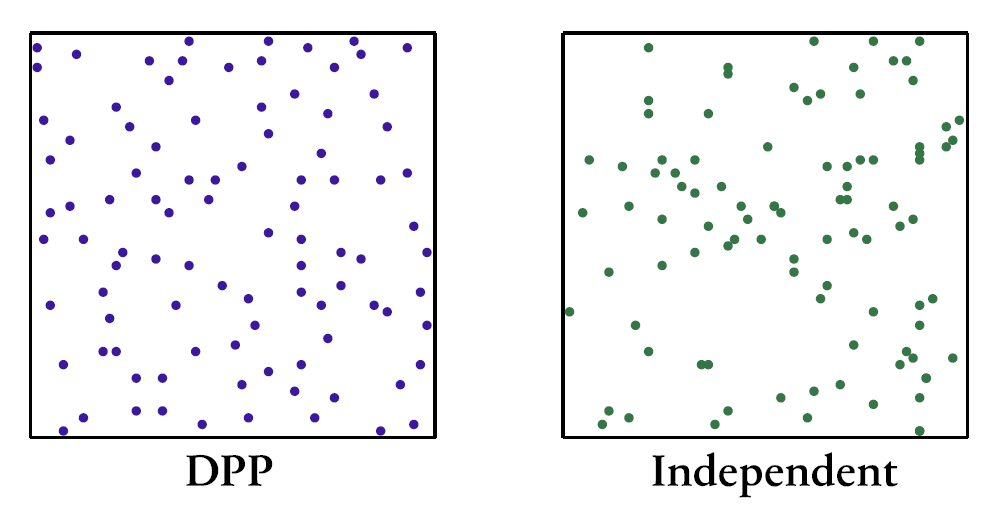
\includegraphics[width=0.6\linewidth]{pics/dpp_vs_iid.png}
    \caption{(left) A set of points in the plane drawn from a DPP, with $K_{x y}$ inversely related to the distance between points $i$ and $j$. (right) The same number of points sampled independently using a Poisson point process , which results in random clumping.}
    \label{fig_dpp_vs_iid}
\end{figure}



\section{Geometric interpretation}
DPPs are defined on determinants, that have an intuitive geometric interpretation. Since a DPP kernel $K$ is symmetric, it exists $V \in \RR^{d \times n}$ such that $K= V V\T$. 
Denote the columns of $V$ by $(V_i)$ for $i\in \intint{1}{n}$. Then $\forall A \subseteq \mathcal{X}$

\begin{equation}
    \PP{}{A \subseteq \mathcal{S}} = \operatorname{Vol}^2(V_A)
\end{equation}

The right hand side is the squared $|A|$-dimensional volume of the parallelepiped
spanned by the columns of $V$ corresponding to elements in $A$.

Intuitively, we can think of the columns of $V$ as feature vectors describing the elements
of $\mathcal{X}$. Then the kernel $K$ measures similarity using dot products between feature vectors, and \cref{def_dpp} says that the probability assigned by a DPP to the inclusion of a set $A$ is related to the volume spanned by its associated feature vectors. This is illustrated in \cref{fig_geometric_interpret}.

\begin{figure}[!ht]
    \centering
    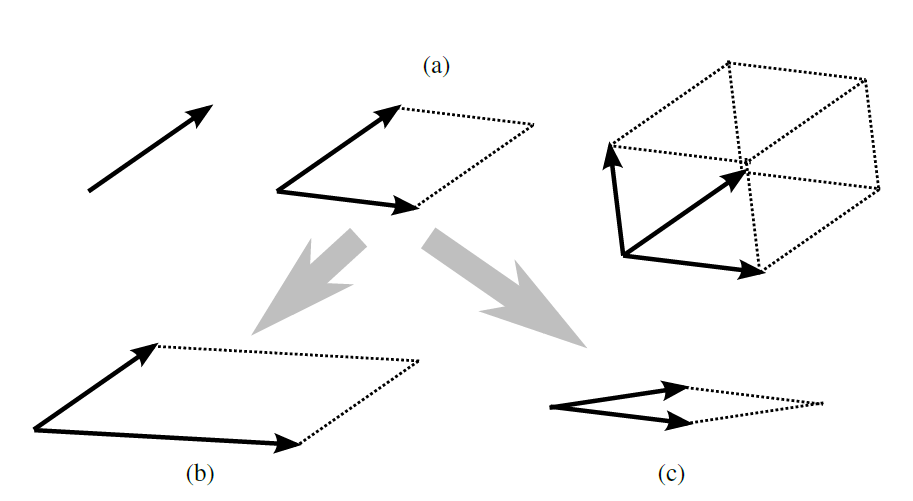
\includegraphics[width=0.8\linewidth]{pics/geometric_interpret.png}
    \caption{from \cite{kulesza2012_dpp_for_ml}. A geometric interpretation of a DPP relates each column of $V$ to an element of $\mathcal{X}$. (a) The  probability of inclusion of a subset $A$ is the square of the volume spanned by its associated feature vectors. (b) As the magnitude of an item's feature vector increases, so do the probabilities of sets containing that item. (c) As the similarity between two items increases, the probabilities of sets containing both of them decrease.}
    \label{fig_geometric_interpret}
\end{figure}

This geometric interpretation explain why diverse sets are more probable. It is because their feature vectors are more orthogonal, and hence span larger volumes. Conversely, items with parallel feature vectors are selected together with probability zero, since their feature vectors define a degenerate parallelepiped. Ceteris paribus, items with large magnitude feature vectors are more likely to appear, because the spanned volume for sets containing them evolves linearly with respect to their magnitude, and thus the probability evolves quadratically with respect to it.


\section{Some useful properties}

projection DPP
mDPP

despite exponential support




\section{Sampling from a DPP}
\subsection{Exact DPP sampling}


Although DPPs can be impressively efficient given the exponential number of subsets being sampled from, sampling can be rapidly limited by performance. 
Except for a few specialised kernels like the edges in uniform spanning trees mentioned previously, the default exact sampler is a spectral algorithm due to \cite{hough2006_hkpv}.

It leverages the fact that DPPs are mixtures of projection DPPs to generate repeated samples given the spectral content of the kernel. This method is commonly called the spectral method since it requires the spectral/eigendecomposition of the positive kernel. 

Formally, if a DPP is defined by a kernel $K$ defined on $n$ data points, one requires the eigendecomposition $K= V V\T$  where $V \in \RR^{d \times n}$. 
This can often be the computational bottleneck since it generally requires $O(n^3)$ time. Note however that for some DPPs based on specific kernels like OPE kernels, $K$ is built via this decomposition and thus it is trivially known.

In any cases when multiple samples are required, this eigendecomposition can be reused. Then each sample from the spectral algorithm requires only $O(n k^2)$ time, where $k$ is the number of elements sampled. This means $O(n (\operatorname{Tr} K)^2)$ time on average. If $K$ is a projection kernel, $k = \operatorname{Tr} K = d$ which is a constant than can be small in many practical applications, e.g. in a recommendation context, $k$ would often be less than 10.

Some recent works from \cite{gillenwater2019_treebased_fast_dpp_sampling} improved somewhat this complexity. Based on the still needed eigendecomposition, it implements a binary tree structure storing appropriate summary statistics of the eigenvectors, requiring $O(n d^2)$ to build, but can then generate repeated
samples in $O(\log(n)k^2d^2 + d^3)$ time, hence $O(\log(n)d^4)$ for a projection kernel.

This method becomes a viable alternative to the spectral method when the total
number of items $n$ is large and when the dimensionality $d$ of the
features and the expected sample size $\operatorname{Tr} K$ are small compared to $n$.





\subsection{Approximate DPP sampling}
Several sampling methods have been developed in the case we only need an approximated DPP sampling.

A first class of methods involves a kernel approximation of a given DPP kernel, using random projections such as in \cite{kulesza2012_dpp_for_ml}, or low-rank factorization techniques.

A second class involves Monte Carlo Markov Chain (MCMC). This is often down in an inexact fashion using target distribution close but different from a DPP one. Noticeably, \cite{gautier2017_zonotope_for_dpp_sampling} proposed an exact MCMC sampler for projection DPPs.

\vspace{10cm}
